% !TeX spellcheck = en_GB

\begin{figure}
	\centering
	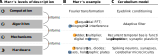
\includegraphics{media/chapters/05_cerebellum/marr_levels.pdf}%
	{\phantomsubcaption\label{fig:marr_levels_a}}%
	{\phantomsubcaption\label{fig:marr_levels_b}}%
	{\phantomsubcaption\label{fig:marr_levels_c}}%
	\caption[Marr and Poggio's levels of description]{Marr and Poggio's levels of description.
	\textbf{(A, B)} Levels of description and corresponding examples from the original paper \citep{marr1976understanding}; coloured numbers highlight different realisations of the same computation.
	\textbf{(C)} Levels of description for our model of eyeblink conditioning.
	}
	\label{fig:marr_levels}
\end{figure}

So far, we have focused on mapping abstract mathematical descriptions onto low-level biological mechanisms.
For example, we have demonstrated that it is possible to compute a variety of mathematical functions while accounting for biological constraints such as Dale's principle.
Furthermore, we showed that synaptic filters and neural dynamics can be exploited to realise temporal bases.
In terms of Marr and Poggio's famous \enquote{levels of description} (quoted on the previous page; cf.~\Cref{fig:marr_levels}; \cite{marr1976understanding}), we have been concerned with levels three and four, that is, thinking about how algorithms can be \enquote{committed} to mechanisms, and how these mechanisms are in turn implemented in a (simulated) neural substrate.

Hence, the primary goal of this chapter is to provide an example of how the methods discussed above can be used to bridge all four levels of abstraction.
Specifically, we implement a simple \enquote{cognitive} system in the form a model of eyeblink conditioning in the cerebellum---starting from the high-level computation (namely \enquote{implementing eyeblink conditioning}) down to the constrained cerebellar microcircuit (\Cref{fig:marr_levels_c}).
Since constructing an intricately detailed model of the entire cerebellum is out of the scope for this thesis, we particularly focus on temporal representations in the Granule-Golgi circuit.

\subsubsection{Implications for cognitive modelling}
Our methodology is remarkably different from the way in which many cognitive scientists and psychologists approach constructing cognitive models.
In these disciplines, models tend to be at the computational and algorithmic levels, and do not explicitly take limitations of the neural substrate into account \citep{eliasmith2015marr}.

Ignoring biological detail can be reasonable depending on the hypothesis that is being explored. 
Yet, as we discussed in \Cref{sec:nef}, a closer look at biology may help in two complementary ways.
First, we can \emph{validate} hypotheses about cognition by determining whether it is possible to implement a particular algorithm in a constrained biological network. 
Second, we can \emph{generate} new hypotheses by asking what class of algorithms a network could support.

We believe that cognitive modellers must ultimately embrace a combination of top-down and bottom-up modelling to narrow down the space of possible cognitive science theories and to direct research attention within that space.
Central roadblocks to the adaptation of this methodology are the availability of modelling tools such as those discussed in this thesis, disseminating information on how to use these tools in practice, and understanding how low-level detail influences high-level function.
Correspondingly, a second goal of this chapter is to study how biological constraints influence \NEF networks on a functional level.

\subsubsection{Implications for neuroscience}
A closed-loop model of eyeblink conditioning in the cerebellum is also interesting from a neuroscience perspective.
It is still unclear how exactly the cerebellum manages to learn and reproduce the timings observed in motor-learning tasks such as eyeblink conditioning.
While earlier theoretical work suggests that the granule cell activities could span a temporal basis \citep{medina2000computer}, this idea has recently come under scrutiny \citep{johansson2014memory}.
To some degree, this is because recordings of the granule activities are scarce, and the source of the hypothesised temporal tuning is unclear.

Understanding how the cerebellum generates timings has far-reaching implications outside motor learning.
Recent evidence---ranging from studies in functional connectivity, neuronal tracing, clinical pathology, to evolutionary physiology---suggests that the same mechanisms are potentially exploited by other cognitive processes as well.
That is, the cerebellum may be recruited by various brain regions as a \enquote{co-processor} to support brain functions related to higher-order cognition, such as language-based thinking, working memory, perceptual prediction, and tasks requiring precise timings in general \citep{sullivan2010cognitive,
           buckner2013cerebellum,
		   oreilly2008cerebellum,
           e2014metaanalysis,
           sanger2020expansion}.

Our experiments suggest that---at least under the constraints we consider---the Granule-Golgi circuit is well-suited to encode temporal information using temporal representations.
This representation can be used in the context of a spiking neural network to learn delays by modulating synaptic weights in the granular-to-Purkinje projection in accordance with the Marr-Albus hypothesis \citep{marr1969theory,albus1971theory,sanger2020expansion}.
These results support earlier simulation work \citep{rossert2015edge}.
We furthermore use our model to generate hypotheses as to why some biological parameters are as observed.

\subsubsection{Structure of this chapter}
The remainder of this chapter is structured as follows.
We first review the eyeblink conditioning task, the particular neurophysiological constraints of the cerebellum, and the theorised mechanisms underpinning delay learning.
We then discuss five neural network implementations with an increasing number of biological constraints, followed by a series of experiments to explore the impact of biological detail on the high-level function.

Finally, we extend our model to the complete eyeblink conditioning task by incorporating the remaining cerebellar microcircuitry, albeit without incorporating quite as much biological detail.
We compare the output of this model to empirical data and show that we are able to---at least qualitatively---reproduce the behaviour of experimental animals.
An overview of our modelling tool NengoBio is provided in \Cref{app:nengo_bio}.